\documentclass{article}
\usepackage{graphicx}
\usepackage[nottoc,numbib]{tocbibind}
\usepackage[a4paper, total={6.75in, 9.25in}]{geometry}
\usepackage{subcaption}
\newcommand{\myparagraph}[1]{\paragraph{#1}\mbox{}\\}

\title{Model-Driven Engineering}
\author{Y1481702}
\date{\today}
\setlength\parindent{0pt}
 
\begin{document}
\begin{titlepage}
\maketitle
\tableofcontents
\end{titlepage}

% This report (MAX 5 pages!) must focus on discussing
%	- how you have interpreted the problem
%	- providing convincing justifications of engineering decisions
%	- convincing examiners that the solution is sound
%	- objectives for the model development

%	- alternative solutions that were considered and the reasons for their rejection
%	- how the work has been tested
%	- why the testing approach was appropriate

% The report must NOT simply describe the solution

\section{Introduction}
\subsection{Objectives}
This report details work in producing model management tools for organising requirements for a large project. This set of tools may be useful for managing requirements in a wide range of projects, both in industry and in academia. The aim is to use domain-specific modeling (DSM), a form of model-driven engineering (MDE), to automate a number of workflows, resulting in productivity gains across a number of projects. These workflows may include tasks such as data validation and auto-generation of a variety of deliverables from application source-code to customer-facing websites. MDE is a software abstraction, we create a specification for a model with its own tools and transformations but need not concern ourselves with the inner workings of these. Abstractions are one of the most important concepts in computer science. As software gets more complex additional abstraction is generally needed in order to extract the most important details of the implementation\cite[p.~24]{csapp}. Previous popular software abstractions, including object-oriented programming, have been shown to result in productivity gains and a better high-level understanding of the software. For instance, attempting to understand the assembly code for a modern application would be incredibly difficult. Model-Driven Engineering has shown promising results in these areas showing that users believe it results in an increase in understanding between stakeholders and can produce productivity gains when models are reused across different projects\cite{industry_review}.

\subsection{Development Process}
Development of this project has roughly followed a quasi-typical MDE process\cite{paige2017changing} using a spiral model approach, returning to the previous stage to adjust the implementation and validation of each requirement as appropriate. Throughout usability testing of the GMF tool, some changes and additions to the metamodel were needed, as discussed in Section \ref{editor}. This is a common occurrence as over the course of a project developers gain an enhanced understanding of the domain which provokes evolution of the metamodel\cite{evolving_models}. Returning to previous stages to alter dependent artifacts can have impact on other work, such as resulting in non-conformance of existing models. \cite{metamodel_sync} categorises metamodel changes and proposes a novel method for resolving some of these issues but this is not yet readily available in standard tools. An alternative approach to MDE, known as flexible modeling, is particularly useful when the model designer is not familiar with MDE. However, these approaches do introduce their own, new problems including lax enforcement of constraints\cite{paige2017changing}.
\\\\
Paige et al. noted that `changing metamodels is a procress that is related to changing programming language APIs'\cite{evolving_models}. I know from first hand experience in industry that changes like this can cause a wide ranging impact. I have had my own software impacted when external APIs have been altered. This project has been assessed to be very small scale, initially at least. As such, any changes to any artifacts, including metamodels, will have no impact outside of the project itself. In the real world, additional care would need to be taken to ensure explicit metamodel versioning, backward-compatibility and time for users to adjust to any updated schema. If the scope of the project changes later on, model migration tools for this purpose could be developed using Epsilon Flock. In industry, a migration tool would be required for any changes to metamodels that have the potential to break its instances. Clearly the development of model migration tools are an overhead specific to MDE. This highlights one of the key difficulties with MDE, particularly with the use of metamodels. It has been proposed that MDE could be performed without metamodels using schemaless XML\cite{evolving_models} but there has not yet been enough work on this matter to justify its use for this project.

\subsection{Code Style}
In order create model code that is mostly self-documenting, I have often elected to use longer names for classes and variables. For example `\texttt{Requirement}' has been used rather than `\texttt{Req}'. While this results in the code being more verbose, it should also be easier to understand and keep the need for comments to a minimum. Using any modern IDE that provides support for auto-completion and refactoring will minimise any additional development overhead caused by this. When naming elements, I also have aimed for internal consistency throughout the project. For example, the project brief uses the term `system requirement' and `technical requirement' interchangeably. In contrast, the project code uses only the former term in order to ensure consistency and avoid confusion.

\subsection{Persistance}
Models in this project are created using the Eclipse Modeling Framework (EMF), this framework stores all models as XML files. This type of representation means that the full model must be loaded into memory, and may result in performance issues on very large models. The models in project are highly unlikely to be large enough to cause problems, therefore this solution is acceptable. If the project scale changes to require very large models, random access strategies may be required to overcome this problem\cite[p.~144]{mdse_in_practice}. mongo-emf claims to be a solution to the that requires very little additional code, and as such can be easily incorporated into the project at a later date\cite{mongo-emf}.
\\\\
A Version Control System (VCS) is a vital part of any software development project allowing for assisted parallel merging, multiple development branches, and effortless roll-back. While I am most familiar with Git from previous software engineering projects, it is not well suited to model-driven engineering as it ignores the graph based nature of models\cite[p.~146]{mdse_in_practice}\cite{evolving_models}. In this project, I haven't needed to support multiple developers or software branches, so its main function has been to store the history of each of my artifacts. As such, the version control system would not necessarily need to have a semantic understanding of the artifacts as they are unlikely to encounter merge-errors. However, I can not rule out the need for this functionality in future development of the project. EMFStore is specifically designed for models and allows for more effective merging and conflict detections of EMF models\cite{emf_store}. As such, all of the artifacts in this project, including all models, meta-models and transformations, have been versioned and archived using EMFStore, throughout the development process.

\section{Abstract Syntax and Constraints}
\label{abstract_syntax}
% Explain how you have arrived at the abstract syntax and any well-formedness constraints for your DSL
%nb. wellformed means it is valid and conforms to its metamodel
%ill-formed means it does not 
I began by formalising the requirements from the brief, as I understood them, by sketching a UML diagram on paper. This helped me turn the natural language specification into a formal definition. While it may have been possible to create this UML diagram electronically and convert it directly into an Ecore metamodel, since the model was not particularly large it seemed easier to implement it directly into Emfatic.
\\\\
One decision that I had to make while making this initial sketch was how to represent some of the requirements as a formal model. For example, the brief specifies two types of requirements: customer requirements and technical requirements. There are three obvious possible options for representing this in the model. Firstly, a boolean attribute could be used to represent whether this is a customer requirement. Secondly, an enumeration attribute could be used to represent the exact type of requirement (customer or system). Finally, and most logically, inheritance could be used to create a designated subclass for each type of requirement. A boolean attribute will take up the least system memory, but this will be so marginal as to be insignificant. Lower memory usage is also an advantage of using an enumeration instead of a creating a designated subclass. However, memory is unlikely to be a significant constraint on modern PCs and this project does not seem like it is necessarily focussed at an embedded system. Inheritance allows for the different behaviours of our Requirements to be built-in to different classes directly, providing the opportunity for better modularity in the code. An example of this, is allowing for conflicts between the same class of requirements to be implemented directly into the ecore metamodel implementation rather than requiring additional Epsilon Validation Language (EVL) constraints, which would simplify the final implementation. When deciding on one of these implementations, it was also important to think about likely future enhancements to the software and the classification of change\cite{metamodel_sync} that would need to occur. If a new category of requirements needs to be added later we want to limit the impact of the change on other artefacts. Using the boolean implementation would be the most likely to cause a breaking and unresolvable change. Inheritance follows the single responsibility principle and hence models will be more robust to changes\cite[p.~95]{martin2002agile}, so this was chosen as the best option.
\\\\
Adding this inheritance creates additional decisions about where attributes such as completion percentage should be stored. Only leaf nodes need to store a percentage attribute and as customer requirements must decompose into at least one system requirement, they should never be used as leaf nodes. System requirements are not always leaf nodes but they may be decomposed further once more detail is known. As such, their implemention needs to be flexible for switching to/from leaf nodes. All the percentages mentioned in the brief are integers, so an additional assumption has been made that this will always be the case.
\\\\
Another challenge faced was deciding which of the requirements should be built into the Emfatic metamodel and which should be implemented as separate EVL constraints. Most multiplicity requirements, such as that `each test-case needs to be verifying \textbf{at least one} technical requirement', have been implemented using Emfatic's multiplicity expression\cite{emfatic_lang} rather than EVL constraints. The only exception to this is the textual requirement description. While the description could be a containment of a 10+ character sequence, this felt unintuitive and would require extra Java code to return a string representation. Thus, it is stored as a single string and the constraint implemented using EVL.
\\\\
Early on, it became obvious that many assumptions would need to be made regarding ambiguous requirements. For example, the brief specifies that each technical requirement needs to originate from at least one customer requirement which leaves open the option for technical requirements to be decomposed from multiple requirements. As this is a university project, there will be no option to ask for clarification on any of these ambiguities so the implementation has been kept as flexible as possible so as to not limit the end-user. This has often made the implementation more tricky, but without being able to further confirm the exact requirements this can't be ruled out as a necessity. Model elements can only belong to one containment reference at a time\cite{containment_faq} so allowing multiple origins means this decomposition attribute cannot be a containment. Ecore requires objects to have some top-level container, so a top-level object class `\texttt{Gathering}' has been created. This will be the main container of all our requirements, team members and test cases. It will need to have a method to access the top level requirements (those with no origin) and an additional EVL constraint will be needed to ensure that system requirements must have an origin. The implementation aims to be simple and intuitive. Attempting to implement constraints such as customer requirements decomposition not being empty and system requirements only decomposing to other system requirements directly in Emfatic would have resulted in a particularly complex metamodel. This type of metamodel would have resulted in a less flexible graphical editor and made model management transformations more difficult to implement. Thus, most of this specification has been implemented by writing EVL constraints to constrain a simple Emfatic metamodel.
\\\\
Opposites are a useful feature of Emfatic allowing for automatically maintained two way links. This is particularly useful for traversing the decomposition tree. It would be useful for conflicting requirements could use opposites in its implementation as this is also a two way relationship. However, at present Ecore, which is the foundation of Emfatic metamodels, does not allow for a reference to be the opposite of itself. This seems to be an unnecessary limitation, and has been the result of multiple discussions for future enhancement on the Eclipse forums\cite{opposite_discussion_1, opposite_discussion_2}. As such, in my implementation this link has been implemented as a standard non-opposite attribute, and EVL validation used to enforce it. An alternative to this solution could have been to have two conflict attributes which are opposites. In order to get a list of all conflicts, they two ELists could be merged. However this data representation has not been used because it is very unintuitive to users unfamiliar with the limitations of Ecore.
\\\\
EVL provides a variety of useful features that have been utilised. Suggested fixes are provided for constraints allowing the user to easily fix problems with their model during the validation process. Critiques have been added for issues in the model that a user may want to be aware of, but were not specified as requirements in the initial brief. Assumptions have been made here with regards to the best practice of data representation, but they follow well-established convention, such as beginning names with a capital letter. In particular, EVL warns when a team member's name does not begin with a capital letter and when no work has been allocated to them.

\section{Editor}
\label{editor}
% Explain the editor for your DSL, justify the decisions you have made
% & briefly argue why your editor provides an appropriate notation for your DSL
%TODO: Sirius/Graphiti as other Graphical Editor options.. GMF uses Graphiti?
EuGENia has been used to implement the editor as it hides the unnecessary complexity of GMF allowing for a graphical editor to be created with minimal work. The editor allows non-technical users to easily create and manage models that conform to the metamodel described in Section \ref{abstract_syntax}. The implementation of the editor has been limited by some of the decisions made when implementing the metamodel. For example, requirements decomposition can only be shown in the editor using a link rather than affixed or a compartment as it has not been stored under containment. Using a compartment would show each high-level customer requirement with the lower-level requirements it is made up of simplifying the diagram by removing the links which often get tangled. Unfortunately, since these lower-level requirements have been allowed to have multiple origins, this display option is not possible in the graphical editor.
\\\\
There may be many cases when multiple team members may have the same forename or surname, so displaying both on the diagram will be the best implementation here. Each name may be required separately and they are, in a sense, two pieces of data and should therefore be stored as such. A derived attribute for full name allows both names to be stored separately and for the full name to appear on the diagram. Adding this attribute required a non-breaking metamodel change. Replacement icons for the GMF editor are available (Fig. \ref{fig:graph_editor}) which help the user distinguish between different nodes on the diagram. These must be incorporated into the GMF editor extension as described in the \texttt{README} file.
\\\\
There is no need for arrows on the links between TeamMembers and Requirements or TestCases and Requirements on the diagram, as this would have no meaning. The items are linked, but there is no implicit directionality here, and it would be wrong for the user to infer such a direction. This is the same for conflicting requirements, if two requirements conflict, this is a two way relationship, so there is no directionality. In constrast to this, arrows are added to the links showing decomposition of requirements. The meaning here is intuitive, it is showing that one requirement is comprised of others. Unfortunately, my implementation of conflicting requirements results in two edges being present on the Graphical Editor, one for each direction of the link, this is not ideal, but is a constraint of the implementation that has been chosen in Section \ref{abstract_syntax}.


\section{Model Management Operations}
% Explain the model management operations for your DSL, justify the decisions that you have made
% Briefly demonstrate that the model management operations can be used to fulfil the model management tasks described in [problem def brief]
Model transformation operations have been implemented as described in the brief. Both of the provided tranformations are good examples of a repetitive, error-prone task that MDE aims to automate. As these transformations make use of the derived attributes in the metamodel, they must be run from a new instance of Eclipse. Additionally, they expect to receive a valid model that conforms to the \texttt{RequirementsGathering} metamodel and its corresponding EVL constraints as discussed in Section \ref{abstract_syntax}.

\subsection{Model-to-Model}
%Generate a simplified requirements model through a model-to-model transformation, which excludes completed requirements as well as team members and use-cases that are only associated to such requirements
\label{model-to-model}
The model transformation removes completed requirements and any associated resources, but the new model may contain all the same model elements- Requirements, Team Members and Test Cases. As such, there is no need for a meta-model change here, both the input and output models will conform to the same metamodel. This transformation is fairly simple to implement, each attribute is simply transferred straight over to the new model. In order to remove the unwanted model elements, guards have been added in the transformation rules to filter out anything that is related to a completed requirement.
\\\\
As this model transformation is intended to by lossy, some issues may appear in the new model due to missing data. Firstly, and most simply, the way that progress is calculated means that by removing any completed requirements progress counters are reset to include only the remaining requirements. There is no requirement in the project specification stating that this is not the desired effect, therefore I have made no attempt to mitigate it. A second, and more major issue, is caused by any conflicting requirements. It's tricky to decide how to handle these occurences. As specified in the brief, if a requirement is completed, any of the requirements that are in conflict with it can no longer be satisfied. As such, if we remove the completed requirement, this constraint would disappear in the new model and we would be unaware of it. If we simply leave it in the model, the requirements it has been decomposed from may also be completed and be removed, potentially invalidating our model. This is a significant problem for the implementation as the exact desired behaviour for this is not mentioned in the brief. The solution for this is was to the user a range of possible fixes if this occurs in the transformation. This has resulted in a more complex implementation, but it can be easily simplified once the desired behaviour is known. One fix has required a new \texttt{insatiable} flag to be added to the metamodel, this metamodel change is non-breaking and so was fairly simple to perform. This flag specifies that a requirement can not be completed as a conflicting requirement has already been completed but removed from the diagram.

\subsection{Model-to-Text}
\label{model-to-text}
%THESE ARE the transformations:
%Generate static HTML website through model-to-text transformation that allows non-modellers to browse through the team members, requirements and test-cases of the system. Users should be able to:
	%Drill down the requirements/test-cases decomposition tree
	%Visualise the progress of requirements in an intuitive way (e.g. through a progress bar)
	%View requirements assigned to particular team members
	%View requirements verified by a specific test case
	%Filter out completed requirements

%INDUSTRY PAPER (J. Hutchinson) discusses 'whether code generation works in practice'
The model-to-text transformation is comprised of a model-to-model transformation which generates an intermediate model conforming to the included Report metamodel, followed by a model-to-text transformation which generates a website from the Report model. This method is a trade-off between automation and flexibility\cite{evolving_models}, while some flexibility may be lost by genericising the second half of the transformation, it has the potentially for significant productivity gains. The webpage generation can be used by models conforming to many different metamodels by implementing the first stage model-to-model transformations into this intermediate model. Then, a wide variety of different output formats can be produced from the intermediate Report model by implementing new model-to-text transformations only once. Thus, this implementation will allow maximum code reuse across different projects, this will hopefully allow an increase in productivity for a relatively minimal additional initial overhead. For ease of use, I have provided an ANT script which will allow these transformations to be run back to back. In the generation of the webpage, I have made the reasonable assumptions that the user be using a modern web browser and have access to the internet. This has allowed me to use modern web-technologies and existing libraries to more easily implement certain requirements, such as progress bars. This significantly reduced the implementation time which was a significant constraint as there was a hard deadline for the project.
\\\\
The homepage of the report lists all of the top-level requirements that every other requirement originates from, as well as a list of all team members and the number of tasks allocated to them. This view will be very useful for the project managers as they will be able to quickly tell how the project is progressing and which team members may have an unsuitable workload. Another notable part of the report is a result of the discussion on requirement conflicts in Section \ref{model-to-model}. As mentioned, there may be cases when requirements can no longer be completed due to a conflicting requirement being completed. In this case, while the model is still valid, the project manager will definitely want to be aware of these points so that they can stop any current or planned work on this requirement. As such, a warning message is placed onto the progress bar of any requirements which cannot be completed. Each generated webpage has a protected region at the top and then below each table, for the user to add their own notes to the generated report. These notes will be preserved if the report is re-generated. By default, I have chosen to leave these regions blank, so that the user does not need to go through each page and delete placeholder text if there are no notes required. Without placeholder text the end user may not become aware of this feature but, providing it is well documented, this should not be a major issue. Page icons used in the model-to-text transformation have been kept consistent with those used in the graphical editor.

\section{Testing and Conclusion}
% Justify the decisions that you have made and how you have tested the AbSyn and constraints
Testing is an important part of any software project and MDE is no exception to this. Manual unit testing is often repetitive and error-prone, exactly the kind of task that MDE aims to automate. The Epsilon Model Generation Language (EMG)\cite{epsilon_book} allows complex models to be semi-automatically generated. An EMG script, along with a selection of models, can be found within the models folder bundled with this report. These bundled models are a mixture of larger automatically generated, and smaller manually created ones. The included EMG script generates well-formed models that conform to both the metamodel and respective constraints, but can and has been modified to generate ill-formed models in order to test that these are rejected in model validation. EUnit tests (not included) have been used to verify the correctness of operations in model transformations.
\\\\
As well as using automatically generated models to ensure that the project is correct and scales to larger projects, usability testing was performed to verify the software's usefulness on a real project. The `\texttt{1.y1481702}' model and it's respective diagram have been attached as evidence of this. These demonstrate the successful usage of the software to track each of the requirements for the MODE Open Assessment. A future enhancement to this model could run EVL validation on any TestCase instances to ensure that the respective EUnit test runs successfully by invoking Java. During the usability testing, I discovered that as the complexity of models goes up, the decomposition and conflict links between requirements becomes very messy. Unfortunately, this is hard to mitigate due to the decision to allow requirements to originate from multiple other higher level requirements in the decomposition tree as containment cannot be used. However, this decision turned out to be helpful in creating the requirements diagram as many of the project requirements interlink.
\\\\
Many of the benefits of MDE do not manifest themselves during the initial implementation but after model reuse, so it's important to view the work in the context of further work\cite{industry_review}.  Facilitating reuse has been the core aim of this implementation and has produced a set of modeling tools which should be easy to maintain and reusable for a range of projects. Thorough testing has ensured these tools fulfil their requirements and are able to scale to reasonably sized models.
\newpage
\raggedright
\bibliography{Report}{}
\bibliographystyle{ieeetran}
\newpage
\section{Appendix}

\begin{figure}[h]
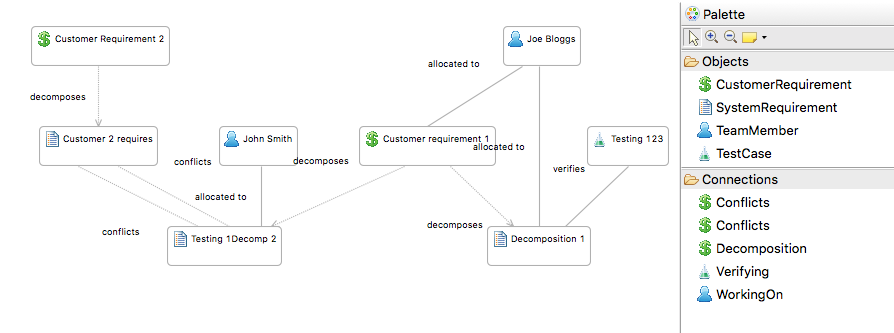
\includegraphics[width=\textwidth]{graphical_editor}
\caption{The Graphical Editor, complete with custom icons for each element.}
\label{fig:graph_editor}
\end{figure}

\end{document}